\label{ch:methods}
We will now

\section{Statistics}
Introduce section

\subsection{Sensitivities}
Neutrino experiments are characterised by the extremely small scattering cross
section of weak processes. Neutrinos are almost massless, have no charge, and
being leptons, they are not affected by strong interactions. These unique
properties make their detection particularly difficult and the associated
experiments particularly costly and time-inefficient. The best way for
experimenters to compensate for a small cross section is to increase the scale
of their detector. 

The Sudbury Neutrino Observatory (SNO) experiment, which confirmed
the existence of matter effects on neutrino oscillations in 2001, consisted of 1000
tons of heavy water enclosed in a sphere of diameter 12 meters\cite{thomson}.
The DUNE experiment, expected to start collecting data in 2024, will use 4850L
of liquid argon for a total fiducial mass\footnote{The outermost parts of the
detector are more sensitive to background events. To account for this, all
events outside the more reliable central region are discarded. The part of the
total detector mass that remains is called fiducial mass.} of 40 kilotons\cite{cdr}.
For projects of this scale, it is crucial to try to maximize the time and cost
efficiency of the experiment by choosing the design that will provide the best
chance of scientific discovery. It is thus conventional as part of the design
process to evaluate the experiment's sensitivity to the relevant physical
parameters. This is then used to legitimize the project to the scientific
community and attract the support of funding agencies.

In general, it is not obvious which design choices (baseline, for example) will lead to better
sensitivity. By sensitivity, we mean the ability of the experiment to make a
relevant discovery. For example, the sensitivity of DUNE to $\delta_{CP}$ is
its capacity to discover CP violation in the lepton sector, i.e. to exclude the
values $\delta_{CP}=0$ and $\delta_{CP}=\pi$ with an acceptable confidence
level.

As a consequence, experimentalists have devised statistical methods to allow
the quantification of sensitivity in order to compare different designs or even
different experiments, and to be able to do so in a mathematically rigorous way that is
accepted by the most scientists.
When applied, these methods enable us to compare potential experiments that
could have different characteristics --- baseline, detector technology,
neutrino source --- and to understand the complementarities that could result
from combining their results.


Currently, one of the most sought after discoveries in neutrino physics is that of the neutrino
mass hierarchy; that is, the sign of the mass difference $\Delta m^2_{31} =
m^2_3 - m^2_1$. Naturally, one can define a statistic that describes how
sensitive a given experiment is to the mass hierarchy. This
statistic will tell us how good the experiment will be at discriminating
between the two possible hypotheses, NH or IH. The larger its value, the more
likely it will be for the experiment's results (for a given run-time) to
provide an answer to the mass hierarchy problem.


\subsection{Derivation of $\Delta \chi^2$ for the mass hierarchy}
The mass hierarchy can only turn out to be normal (NH), or inverted (IH). As
such, it is considered as a discrete, non-nested hypothesis (in contrast with a continuous
variable such as $\delta_{CP}$ or $\theta_{23}$) in our statistical analysis.
The method we use\cite{ciuffoli, qian} is presented in a fairly
statistics-heavy manner but we only use it in its simplest occurence,
namely a model with no nuisance parameters ((this sentence is bad)). However,
we later introduce systematic uncertainties by hand by modeling the
reconstruction of neutrino energies at the detector.

(( This explanation is not well written dude please))
In a neutrino experiment such as DUNE, neutrino events (e.g.~$\nu_e$
appearance) will be recorded as a
function of their reconstructed energy. We denote by $y_i$ the event count per
energy bin,
where $i = 1, 2, ..., N$ is the index of the energy bin.
Given that enough data has been collected,
the event counts $y_i$ will be distributed around the true count
according to a Gaussian with variance $\sigma_i=\sqrt{y_i}$. 
Our theoretical models will yield predicted event counts that will depend on
the true mass hierarchy.  We denote by $y^N_i$ the predicted count under normal
hierarchy and by $y^I_i$ the predicted count under inverted hierarchy.
Let us assume that the true hierarchy (the one picked by nature) is normally
ordered. Then we can write our experimental event counts as $y_i = y^N_i +
\sigma_i g_i$, where $g_i$ is a random variable from a Gaussian distribution
centered at zero and with variance 1.
The $\Delta \chi^2$ statistic can then be written as
\begin{align*}
	\Delta \chi^2 &= \chi_I^2 - \chi_N^2\\
	&= \sum_i \frac{(y_i - y^I_i)^2}{\sigma_i^2} - \sum_i \frac{(y_i -
	y^N_i)^2}{\sigma_i^2}\\
	&= \sum_i \frac{(y^N_i + \sigma_i g_i - y^I_i)^2 - (y^N_i + \sigma_i g_i -
	y^N_i)^2}{\sigma_i^2}\\
	&= \sum_i \frac{(y^N_i - y^I_i)^2}{\sigma_i^2} + \sum_i \frac{2(y^N_i -
	y^I_i)}{\sigma_i} g_i
\end{align*}
In this form, we can see that $\Delta \chi^2$ is a Gaussian-distributed random
variable where the mean is
$$\overline{\Delta\chi^2} = \sum_i \frac{(y^N_i - y^I_i)^2}{\sigma_i^2},$$
and the standard deviation is
$$\sigma_{\Delta\chi^2} = \sqrt{\sum_i \frac{4(y^N_i - y^I_i)^2}{\sigma_i^2}}\\
= 2\sqrt{\overline{\Delta\chi^2}}.$$

In these expressions, the experimental counts $y_i$ do not appear, which means
that we can evaluate the $\overline{\Delta\chi^2}$ (mean delta chi-squared)
statistic from our theoretical models only.

((TODO this is not true, fix))
It is fairly evident\cite{qian} that when the
event count $y^N_i$ is large (we are still under our assumption that the true hierarchy
is normal), we can substitute the statistical uncertainty $\sigma_i$ by
$\sqrt{y^N_i}$, such that our expression becomes
$$\overline{\Delta\chi^2} = \sum_i \frac{(y^N_i - y^I_i)^2}{y^N_i}.$$
If we work under the opposite assumption, where we have a true inverted
hierarchy, the denominator is simply replaced by $y^I_i$. 

This statistic is used throughout the neutrino physics literature\cite{cdr,
martin-albo}((MORE CITATIONS NEEDED)) to express the sensitivity of future experiments.
((Give details)).



\subsection{Sensitivity to $\delta_{CP}$}
In addition to the sensitivity to the mass hierarchy, we estimate the
sensitivity to CP discovery by simulating data for all values of $\delta_{CP}$
and comparing to CP-conserving values $\delta_{CP} = 0, \pi$.

\section{Neutrino oscillations model}
By implementing the concepts introduced in the previous chapter, we are able to
model the oscillation of neutrinos through a vacuum or through matter.

The first step of our work was to implement in code the phenomenological
oscillation formulae of chapter~\ref{ch:introduction}. The simplest test case
is equation~\ref{eq:twonu}, the oscillation between two neutrino flavours.
Figure~\ref{fig:twonu_plots} shows the oscillation
probability of a neutrino initially produced as a $\nu_\mu$. 
\begin{figure}
	\centering
	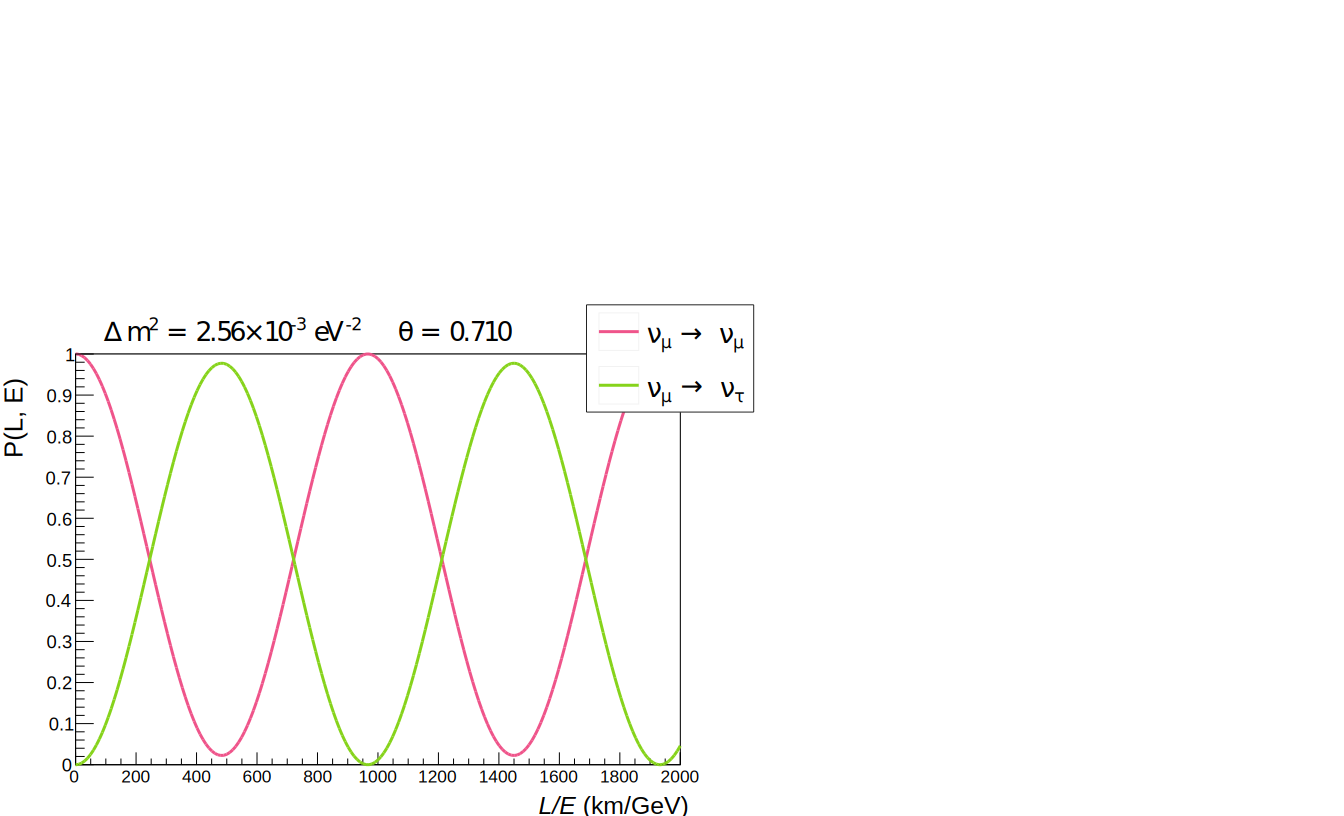
\includegraphics[width=0.6\textwidth]{twonu.pdf}
	\captionsetup{width=0.9\textwidth}
	\caption{Oscillation probability vs. $L/E$ for two neutrino flavours. The
	amplitude is governed by $\theta$ while the frequency is proportional to
	$\Delta m^2$. The mixing between flavours is almost maximal, i.e. the
	appearance of $\nu_\tau$ is almost 100\% at the half period.}
	\label{fig:twonu_plots}
\end{figure}
For this plot, we picked the parameters $\Delta m^2$ and $\theta$ (shown in
figure) from global fits of past experiments, reported by the Particle Data
Group (PDG)\cite{pdg}.

\begin{wraptable}{r}[2cm]{0.36\textwidth}
	\captionsetup{justification=centering}
	\centering
\begin{tabular}{ | c | c | }
	\hline
	Parameter & Value\\\hline
	$\Delta m^2_{21}$ & \SI{7.37e-5}{\eV^{-2}}\\
	$|\Delta m^2_{31}|$ & \SI{2.56e-3}{\eV^{-2}}\\
	$\theta_{12}$		  & 0.576\\
	$\theta_{23}$			& 0.710\\
	$\theta_{13}$ 		& 0.147\\\hline
\end{tabular}
	\caption{Parameter values used in fig.~\ref{fig:threenu_plots} and
	fig.~\ref{fig:dune_prob}}
	\label{tab:threenu_params}
\end{wraptable}

The next step is to implement three-neutrino oscillations. This involves
implementing the complex PMNS matrix of eq.~\ref{eq:PMNS} and the more general
probability function of eq.~\ref{eq:nuprob}. 
\begin{figure}
	\centering
	\makebox[1\textwidth][c]{
		\centering
	\begin{subfigure}[b]{0.6\textwidth}
		\centering
		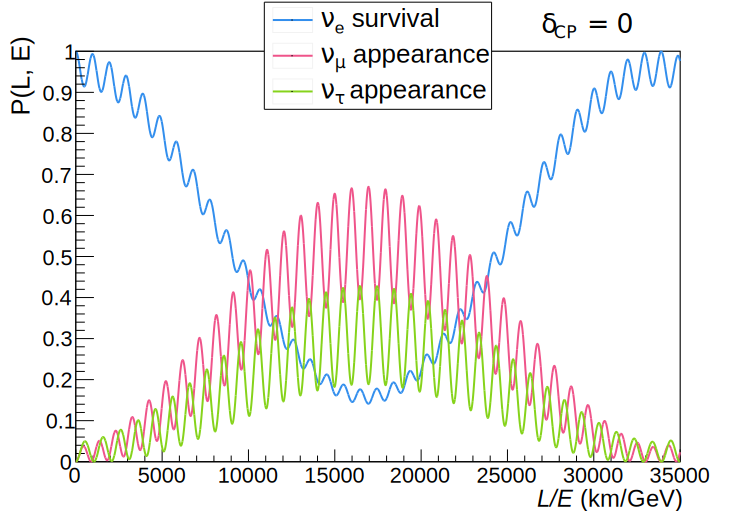
\includegraphics[width=\textwidth]{threenu_0.pdf}
	\end{subfigure}
	\begin{subfigure}[b]{0.6\textwidth}
		\centering
		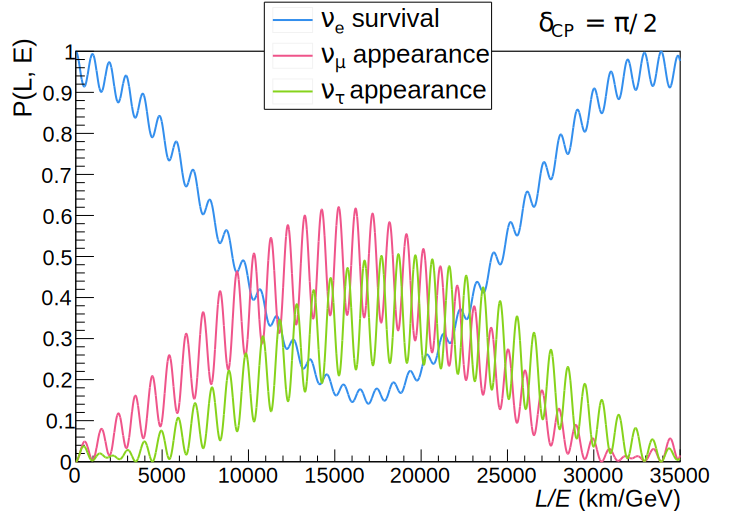
\includegraphics[width=\textwidth]{threenu_pihalf.pdf}
	\end{subfigure}}
\caption{Oscillation probability for a neutrino produced as a $\nu_e$, allowed to
	oscillate to $\nu_\tau$ and $\nu_\mu$. The mass hierarchy is NH for both
	plots. We illustrate the difference made by
	the CP-violating phase by showing a plot where CP is conserved
	($\delta_{CP}=0$) and a plot where CP is maximally violated ($\delta_{CP} =
	\pi/2$).}
\label{fig:threenu_plots}
\end{figure}
Figure~\ref{fig:threenu_plots} shows the oscillation probability for a neutrino
starting as a $\nu_e$ as a function of $L/E$. All parameters except
$\delta_{CP}$ are best-fit values listed by the PDG\cite{pdg} under the
assumption that the true mass hierarchy is normally ordered.
Table~\ref{tab:threenu_params} shows these values.


The difference between the two plots in figure~\ref{fig:threenu_plots} clearly
shows that given all other parameters, it is possible to determine the true
value of $\delta_{CP}$ by measuring neutrino appearance rates. Unfortunately,
the problem is not that easily solved. In neutrino experiments, reconstructing
the energy of neutrinos in the detector is difficult and prone to random and
systematic errors. Additionally, while some parameters are known with good
precision ($\theta_{12}, \theta_{13}, \Delta m^2_{21}$), the others remain
elusive and challenging to measure independently of each other.
Corrections must also be applied when the oscillations take place
through matter. It is necessary to choose an appropriate and reliable model of the
of the medium through which the neutrinos propagate, since the potential $V_e$ of
equation~\ref{eq:matter_potential} is proportional to the electron density in
the medium.


\section{Modelling an accelerator-based long baseline experiment}

\subsection{Intro to DUNE}
The Deep Underground Neutrino Experiment (DUNE) is a future long-baseline
experiment designed to --- among other goals --- determine the CP violating phase
$\delta_{CP}$, the neutrino mass hierarchy (the sign of $\Delta m^2_{31}$) and
the octant of $\theta_{23}$ (whether it is greater or less than 
$\pi/4$)\cite{cdr}. 
It will make use of Fermilab's Long-Baseline Neutrino Facility (LBNF) in Batavia,
Illinois for the production of a high-intensity neutrino beam aimed at the
Sanford Underground Research Facility, \SI{1300}{\km} away, where the DUNE
detectors will be built.
Four liquid argon time-projection chambers (LArTPC) of fiducial mass
\SI{10}{\kt} each will serve as detectors, with the ability to reconstruct the
trajectories and kinematic quantities of interacting neutrinos.
DUNE will primarily observe the oscillations from $\nu_\mu$ to $\nu_e$ in the
LBNF beam. This appearance channel alone is expected to provide enough data to
reach the objectives mentioned above, as we will show later.
The neutrino beam will travel through the Earth's crust for \SI{1300}{\km},
hence matter effects must be taken into account.

The DUNE experiment is thus a perfect candidate to try our simple model and see if
we can reproduce results from the literature, namely predictions on the
potential outcomes of the experiment.

\subsection{Event rate at the detector}
In order to predict an event rate $N$ in a general detector, we usually need three
elements: the luminosity of the beam $L$, the interaction cross section $\sigma$, and the
efficiency of the detector $\eps$:
\begin{equation}N = \eps L \sigma,\label{eq:rate}\end{equation}
where $L$ has units \si{\m^{-2} \s^{-1}}, $\sigma$ has units \si{\m^2} and
$\eps$ is unitless.
We will use a modified version of this approach to predict event rates inside
DUNE's liquid argon time-projection chamber (LArTPC), as a function of
energy. While our model
accurately describes the flavour oscillations of neutrinos, we are unable to
estimate the neutrino flux coming out of the LBNF accelerator, or the
efficiency of the LArTPC. For these two aspects we will rely on results
presented by the DUNE collaboration in their conceptual design report (CDR).

To produce the neutrinos, the LBNF accelerates protons which collide with a
graphite target to produce secondary mesons ($\pi^+, \pi^-$). These particles are focused
along a decay pipe where they decay into muons and their associated muon
neutrinos\cite{papadimitriou}. Hence by modelling the proton/target collision and the
decay of secondary mesons, one can estimate the flux of neutrinos produced by
the accelerator. The volume 3 of the CDR\cite{cdr_vol3} provides the predicted
flux of $\nu_\mu$ and $\nu_e$ at the detector in the absence of oscillations.
To produce these results, they use the \textsc{Geant4}\cite{Geant4} software to simulate
the beamline from the reference design of the LBNF accelerator.
Figure~\ref{fig:nuflux} shows a reproduction of the resulting plot from the DUNE CDR.
\begin{figure}
	\centering
	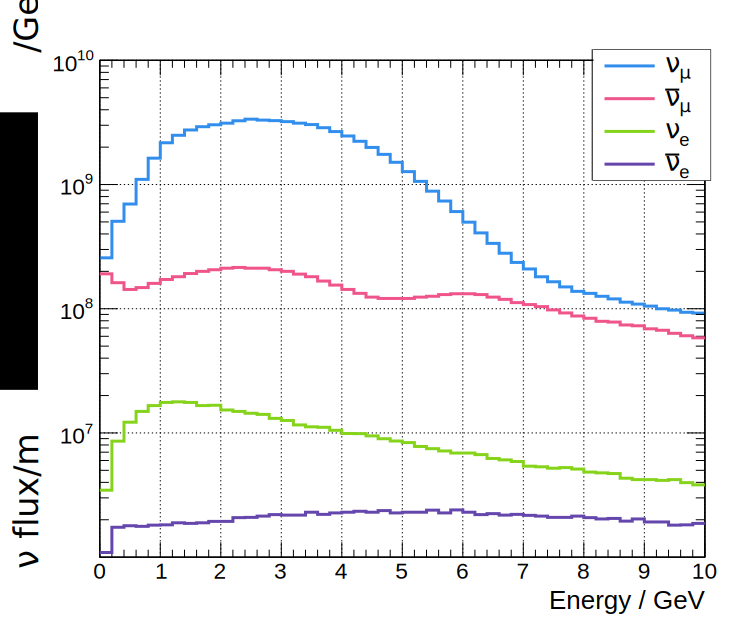
\includegraphics[width=0.5\textwidth]{dune_flux.pdf}
	\caption{Predicted neutrino flux at the DUNE detector in the absence of
	oscillations, when focusing positively charged pions through the decay pipe. 
	``POT'' stands for protons on target.
	Reproduction of figure 6-2 from the DUNE CDR Vol.
	3\cite{cdr_vol3}.}
	\label{fig:nuflux}
\end{figure}

It is fairly simple to convert this ``un-oscillated'' spectrum into an
``oscillated'' one. Typically in accelerator-based experiments, the observed oscillation channel
is the $\nu_\mu \rightarrow \nu_e$ appearance. Hence for each bin in the
spectrum of figure~\ref{fig:nuflux}, we multiply the un-oscillated
muon-neutrino flux
$\Phi^{(\mu)}_0$ (blue line) by the $\nu_\mu \rightarrow \nu_e$ oscillation
probability:
\begin{equation}
	\Phi^{(e)}_\text{osc} (E_i) = P_{\nu_\mu \rightarrow \nu_e} (E_i) \times
\Phi^{(\mu)}_0 (E_i),\label{eq:flux}\end{equation}
where $\Phi^{(e)}_\text{osc}$ is the flux of electron-neutrinos resulting from
$\nu_\mu$ oscillations, and $i$ indexes energy bins.
We show this $P_{\nu_\mu \rightarrow \nu_e}$ function for different values of
$\delta_{CP}$ and the two possible mass hierarchies on
figure~\ref{fig:dune_prob}. We also illustrate the influence of matter effects
on the appearance probability by showing oscillations in vacuum and in the
Earth's mantle.
\begin{figure}
	\centering
	\makebox[\textwidth][c]{
		\begin{subfigure}{0.6\textwidth}
		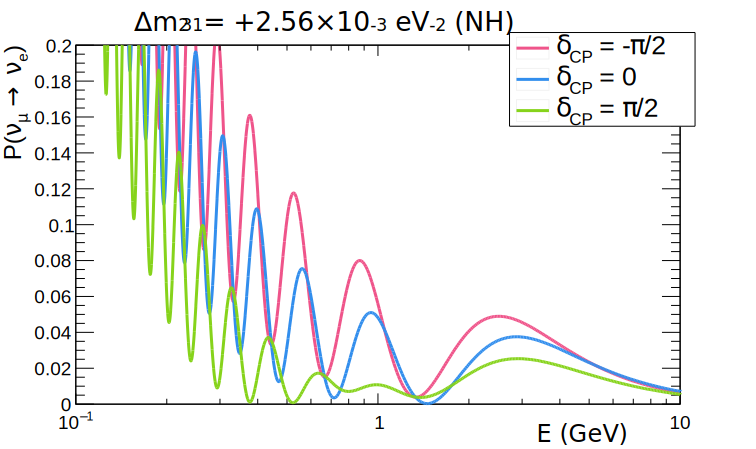
\includegraphics[width=\textwidth]{dune_prob_nh_vac.pdf}
			\caption{Vacuum, NH}\label{fig:vacNH}
		\end{subfigure}
		\begin{subfigure}{0.6\textwidth}
		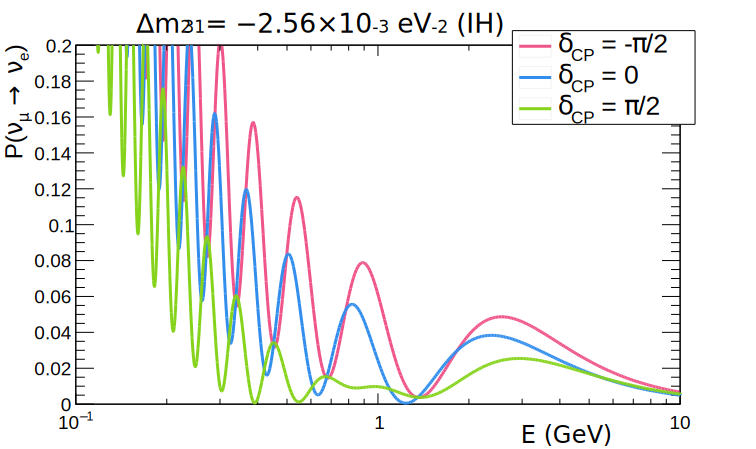
\includegraphics[width=\textwidth]{dune_prob_ih_vac.pdf}
			\caption{Vacuum, IH}\label{fig:vacIH}
		\end{subfigure}}
	\makebox[\textwidth][c]{
	\begin{subfigure}{0.6\textwidth}
		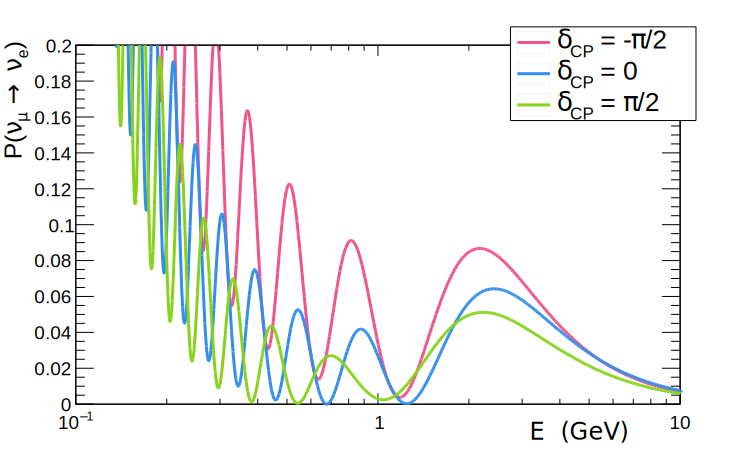
\includegraphics[width=\textwidth]{dune_prob_nh.pdf}
		\caption{Matter, NH}\label{fig:matNH}
		\end{subfigure}
		\begin{subfigure}{0.6\textwidth}
		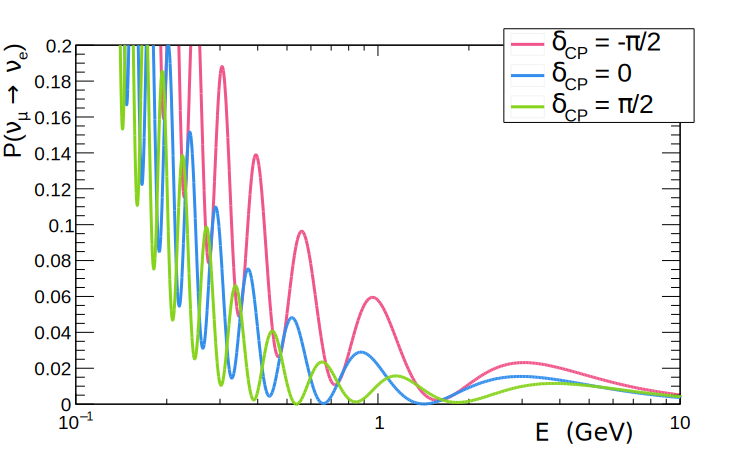
\includegraphics[width=\textwidth]{dune_prob_ih.pdf}
			\caption{Matter, IH}\label{fig:matIH}
		\end{subfigure}}
	\caption{Oscillation probability $\nu_\mu \rightarrow \nu_e$ as a function of
	neutrino energy for neutrinos travelling over a baseline $L=\SI{1300}{\km}$.
	Plots on the left have a normally ordered mass hierarchy, and plots on the
	right an inverted mass hierarchy. On top, neutrinos are oscillated in empty
	space, and on the bottom they are oscillated through matter of constant
	density $N_e=2.2 N_A~\si{\cm^{-3}}$, where $N_A$ is Avogadro's
	constant((citation needed)). All vacuum oscillation parameters are
	listed in table~\ref{tab:threenu_params}.}
\label{fig:dune_prob}
\end{figure}

In general, the first (rightmost) peak\footnote{It is the ``first peak''
because the probability falls to zero at higher energies. Note that the curves
in figure~\ref{fig:threenu_plots} had $L/E$ on the x-axis, while those in
figure~\ref{fig:dune_prob} are plotted against $E$. Hence the region covered by
the latter corresponds to the leftmost part of the former.} in the oscillation
probability will provide the best signal, since it is wider than all other
peaks on the energy axis, and thus easier to resolve.
The first oscillation peak for the DUNE baseline $L=\SI{1300}{\km}$ occurs between 1 and
\SI{10}{\GeV}, and thus it is the
energy range of choice for the DUNE experiment\cite{cdr}. 

It is interesting to observe that matter effects enhance the amplitude of
oscillations for the NH, and reduce it for the IH. The mass hierarchy only
influences the sign of one of the mass-squared differences, thus in a vacuum it
only affects the frequency of oscillations, as is shown on
figures~\ref{fig:vacNH} and~\ref{fig:vacIH}: the peak amplitudes are left
unchanged under a change of hierarchy. In vacuum, we can only change the
amplitude by changing the mixing angles. We see on figures~\ref{fig:matNH}
and~\ref{fig:matIH} that matter effects mix the parameters --- as is manifest
already for two neutrinos in equation~\ref{eq:deltam2m} --- in such a way that the
mass hierarchy can impact the amplitude as well. This feature is crucial to
DUNE's sensitivity to the mass hierarchy, as it will make discriminating
between the two hypotheses much easier than if the neutrinos were propagating
in empty space.

Now that we have the neutrino flux in the detector, i.e.~the luminosity
variable of equation~\ref{eq:rate}, we would normally need a model of the weak
interactions with the liquid argon ($\sigma$) and of the detector efficiency
($\eps$).
However another option is to normalize the flux to the integrated event rate,
i.e.~the total number of events expected to be observed during a given exposure
time. If we denote by $N_\text{int}$ this integrated event rate, then the
predicted event rate per unit energy is
\begin{equation}
	\frac{\md N}{\md E} = \frac{N_\text{int}}{\int \Phi^{(e)}_\text{osc} (E)~\md E}
	\times \Phi^{(e)}_\text{osc} (E).
\end{equation}
In other words, we first normalize the flux spectrum $\Phi^{(e)}_\text{osc}$ to
1 by dividing it by its integral, and then normalize to the integrated event
rate by multiplying by $N_\text{int}$.
Since our flux is a function of discrete energy bins, we can rewrite this as
\begin{align}
	\frac{N_i}{\Delta E} &= \frac{N_\text{int}}{\sum\limits_j \Phi^{(e)}_\text{osc} (E_j)
	\Delta E} \times \Phi^{(e)}_\text{osc} (E_i)\nonumber\\\implies
	N_i &= \frac{N_\text{int}}{\sum\limits_j \Phi^{(e)}_\text{osc} (E_j)} \times
	\Phi^{(e)}_\text{osc} (E_i),\label{eq:event_rate_0}
\end{align}
where $N_i$ is now the event rate per energy bin.
Thus, from the integrated event rate, we are able to retrieve the event rate as
a function of energy. We can then use this data to obtain the experiment's
sensitivity to the mass hierarchy and $\delta_{CP}$.

The CDR uses the \textsc{Genie}\cite{GENIE} neutrino event generator and a
parametrized detector response, to process the neutrino flux and
obtain an event rate through Monte Carlo simulations. This complex modelling
allows them to ``classify the types of neutrino interactions, including
backgrounds and misidentified interactions''\cite{LBNE}. 
Hence they are able to predict that the total number
of CC events from $\nu_e$ appearance between 0.5 and \SI{8}{\GeV} during an exposure of 150
kt$\cdot$MW$\cdot$year will be $N^{N}_\text{int}=861$ if the true hierarchy is normal,
and $N^{I}_\text{int}=495$ if it is inverted. Although both results assume that
$\delta_{CP}=0$, we will be able to calculate the event rates for all values of
$\delta_{CP}$ using our model.

As can be seen on any of the graphs of figure~\ref{fig:dune_prob}, the area under the first
appearance peak is different for different values of $\delta_{CP}$. This
indicates that the integrated event rate depends on $\delta_{CP}$.
The integrated event rate for any $\delta_{CP}$ is given by
\begin{align}
	N_\text{int} (\delta) &= \frac{\int P (
	\delta)~\md E}{\int P (
	\delta=0)~\md E} \times N_\text{int}\nonumber\\
		&= \frac{\sum_j \Phi_j (\delta) }{\sum\limits_j \Phi_j (\delta=0)} \times
	N_\text{int},\quad\text{using eq.~\ref{eq:flux},}\nonumber
\end{align}
where $P(\delta)$ is the $\nu_\mu\rightarrow\nu_e$ appearance probability
for any $\delta_{CP}=\delta$, and $\Phi_j \equiv \Phi^{(e)}_\text{osc}(E_j)$.
Thus, substituting into equation~\ref{eq:event_rate_0},
\begin{align}
	N_i (\delta) &= \frac{N_\text{int}(\delta)}{\sum\limits_j \Phi_j (\delta)}
	\times \Phi_i (\delta)\nonumber\\
	&= \frac{N_\text{int}}{\sum\limits_j \Phi_j (\delta)} \frac{\sum_j \Phi_j
	(\delta)}{\sum\limits_j \Phi_j (\delta=0)} \times \Phi_j(\delta)\nonumber\\
	&= \frac{N_\text{int}}{\sum\limits_j \Phi_j (\delta=0)} \times
	\Phi_j(\delta).\label{eq:event_rate}
\end{align}
Equation~\ref{eq:event_rate} allows us to calculate an event rate spectrum
for any $\delta_{CP}$ using the integrated event rate from the CDR and two
predicted fluxes we calculate using eq.~\ref{eq:flux}.
Figure~\ref{fig:event_rate} shows examples of such spectra, for two values of
$\delta_{CP}$ and the two possible hierarchies.



\begin{figure}
	\centering
	\makebox[\textwidth][c]{
	\begin{subfigure}{0.6\textwidth}
	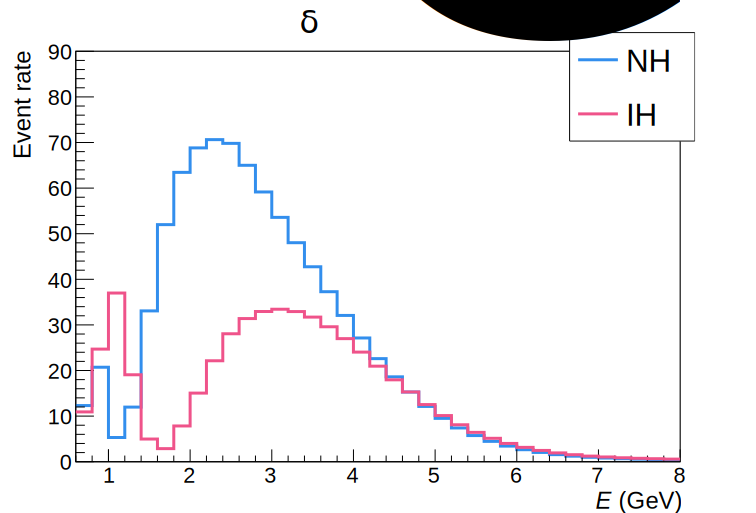
\includegraphics[width=\textwidth]{event_rate_0.pdf}
	\end{subfigure}
	\begin{subfigure}{0.6\textwidth}
		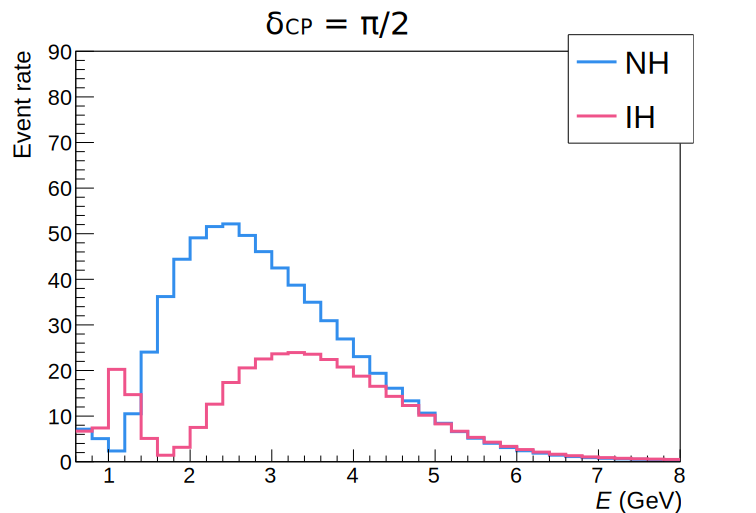
\includegraphics[width=\textwidth]{event_rate_pi.pdf}
	\end{subfigure}
	}
	\caption{Predicted event rate at DUNE as a function of neutrino energy, for
	two values of $\delta_{CP}$ and the two hierarchies.}
\label{fig:event_rate}
\end{figure}

\subsection{Energy reconstruction}





